%----------------------------------------------------------------------------------------
%    Đề tài: Theo doi cong suat cua phu tai mot pha
%
%    Thực hiện: Thi Minh Nhut - Huynh Nhu - Nguyen Thi Anh Thu
%
%    Build: pdflatex -- pdflatex -- View PDF
%
%    Thời gian: Ngày 10 tháng 12 năm 2017
%
%----------------------------------------------------------------------------------------

% Sử dụng fontsize 13pt, khổ giấy đứng A4 với lớp mở rộng của lớp report
\documentclass[13pt,a4paper]{extreport}

%% Cho phép biên dịch tiếng Việt trong LaTeX
\usepackage[utf8]{inputenc}
\usepackage[utf8]{vietnam}

% Sử dụng font chữ Times New Roman
\usepackage{times}

% Gói lệnh thao tác đến các công thức toán
\usepackage{amsmath}
\usepackage{amsfonts}
\usepackage{amssymb}

% Tự động thụt vào đầu dòng cho mỗi đoạn
\usepackage{indentfirst}

% Định dạng lề văn bản
\usepackage[left=3.5cm,right=2cm,top=3cm,bottom=3cm,headsep=.15in]{geometry}

% Gói lệnh cho phép thao tác với hình ảnh
\usepackage{graphicx}        % trim option ={<left> <lower> <right> <upper>}
\usepackage{subfig}
\graphicspath{
    {images/esp8266/}
    {images/smartconfig/}
    {images/arduino-ide/}
    {images/blynk/}
    {images/thingspeak/}
    {images/acs712/}
    {images/result/}
    {../flowchart/}
    {../schematic/}
    {cover/}
}

% Tùy chỉnh style trong caption
\usepackage[labelfont={it}, textfont={it}, skip=0pt]{caption}    % Định nghĩa style cho caption
\setlength{\belowcaptionskip}{-10pt}        % Giảm khoảng cách từ caption đến text


% Gói lệnh vẽ hình
\usepackage{tikz}
\usetikzlibrary{arrows, decorations.markings, calc, fadings, decorations.pathreplacing, patterns, decorations.pathmorphing, positioning}

% Gói lệnh vẽ lưu đồ giải thuật
\usepackage{flowchart}

% Gói lệnh cho phép chèn code từ bên ngoài vào tài liệu
\usepackage{listings}
\lstset{frame=tb,
    frame=none,
    aboveskip=3mm,
    belowskip=3mm,
    showstringspaces=false,
    columns=flexible,
    basicstyle={\small\ttfamily},
    breaklines=true,
    breakatwhitespace=true,
    tabsize=4,
    inputpath={../code/acs712_arduino/}
}


% Chèn file tex từ ngoài vào tài liệu và bỏ đi phần đầu
\usepackage[subpreambles=true]{standalone}
\usepackage{import}

\usepackage{verbatim}

% Thêm chữ chương vào mục lục
\usepackage{titletoc}%
\titlecontents{chapter}% <section-type>
    [0pt]% <left>
    {\bfseries}% <above-code>
    {\chaptername\ \thecontentslabel\quad}% <numbered-entry-format>
    {}% <numberless-entry-format>
    {\hfill\contentspage}% <filler-page-format>
\usepackage[hidelinks=true,
            pdfproducer={Mircosoft Office},
            pdfcreator={Mircosoft Office}]{hyperref}
%%% Tạo Headers và footers
\usepackage{fancyhdr}
\pagestyle{fancy}
\fancyhf{}
\renewcommand{\headrulewidth}{1.2pt}
\renewcommand{\footrulewidth}{1.2pt}

\fancyhead[L]{\textit{\leftmark}}
\fancyfoot[L]{\textit{Đồ án Hệ thống điện}}
\fancyfoot[R]{\thepage}
\fancypagestyle{plain}{%
    \renewcommand{\headrulewidth}{0pt}%
    \renewcommand{\footrulewidth}{0pt}%
    \fancyhf{}%
    \fancyfoot[R]{\thepage}%
}

% Chế độ gõ công thức toán trên một dòng
\everymath{\displaystyle}

\renewcommand{\baselinestretch}{1.2}    % Giản dòng
\setlength{\parskip}{6pt}    % Khoảng cách giữa các đoạn

% Định nghĩa một số lệnh và môi trường mới

% Dùng khi tham chiếu hình ảnh
\newcommand{\fig}[1]{Hình~#1}
% Tạo khoảng trống phía sau đơn vị
\newcommand{\unit}[1]{~#1}
% Tạo một trang trống
\newcommand*\NewPage{\newpage\null\thispagestyle{empty}\newpage}

%----------------------------------------------------------------------------------------
%
%    Nội dung chính của tài liệu nằm trong \begin{document} và \end{document}
%
%----------------------------------------------------------------------------------------

\begin{document}

    %----------------------------------------------------------------------------------------
    %    Trang bìa
    %----------------------------------------------------------------------------------------
    \pagenumbering{gobble} % Không đánh số trang cho trang bìa
    \newgeometry{left=3.5cm,right=2cm,top=3cm,bottom=3cm,headsep=.15in}
    %----------------------------------------------------------------------------------------
%    TITLE PAGE
%    Tham khảo: https://www.overleaf.com/10408157zrdwddmpddkf#/38720772/
%    Tham khảo: https://www.latextemplates.com/template/academic-title-page
%----------------------------------------------------------------------------------------

\begin{titlepage} % Suppresses displaying the page number on the title page and the subsequent page counts as page 1
    \begin{tikzpicture}[remember picture, overlay]
        \draw[line width = 3pt] ($(current page.north west) + (1.2in,-.75in)$) rectangle ($(current page.south east) + (-.65in,.75in)$);
    \end{tikzpicture}
    \newcommand{\HRule}{\rule{\linewidth}{0.5mm}} % Defines a new command for horizontal lines, change thickness here

    \center % Centre everything on the page

    %------------------------------------------------
    %	Headings
    %------------------------------------------------
    \vspace*{-1.5cm}
	{\large\bfseries TRƯỜNG ĐẠI HỌC \\ KỸ THUẬT -- CÔNG NGHỆ CẦN THƠ} \\ % Main heading such as the name of your university/college
	{\large\bfseries KHOA ĐIỆN -- ĐIỆN TỬ -- VIỄN THÔNG} \\ [1cm]

    %------------------------------------------------
    %    Logo
    %------------------------------------------------
    
\includegraphics[width=0.2\textwidth]{logo_ctut.pdf} \\ [.5cm] % Include a department/university logo - this will require the graphicx package

    {\LARGE\bfseries ĐỒ ÁN HỆ THỐNG ĐIỆN} \\ [0.5cm] % Major heading such as course name

    %\large{Minor Heading}\\[0.5cm] % Minor heading such as course title

    %------------------------------------------------
    %    Title
    %------------------------------------------------

    \vspace*{0.4cm}
    % \HRule\\[0.4cm]

    {\Large \bfseries ĐỀ TÀI \\ [0.2cm] THEO DÕI ĐIỆN NĂNG TIÊU THỤ CỦA PHỤ TẢI MỘT PHA VỚI CẢM BIẾN DÒNG ACS712} \\ [0.4cm] % Title of your document

    % \HRule\\[1.0cm]

    \vspace*{1.0cm}

    %------------------------------------------------
    %	Author(s)
    %------------------------------------------------


    \begin{tabular}{ll}
        \multicolumn{2}{l}{{\large Giảng viên hướng dẫn: \quad Huỳnh Nguyễn Xuân Cần}}\vspace{.3cm}\\
        \multicolumn{2}{l}{{\large Lớp: \quad Công nghệ kỹ thuật điện, điện tử  2014-2}}\vspace{.3cm}\\
        {\large Nhóm sinh viên thực hiện:} &\vspace{.2cm}\\
        {\large \hspace{1.5cm} 1. Huỳnh Như (MSSV:  1400012)}& \vspace{.2cm}\\
        {\large \hspace{1.5cm} 2. Nguyễn Thị Anh Thư (MSSV: 1400450)}& \vspace{.2cm}\\
    \end{tabular}


    %------------------------------------------------
    %	Date
    %------------------------------------------------

%    \vfill\vfill

%    {\large\bfseries (Version TK-HTD-1.0.0)}

    \vfill\vfill % Position the date 3/4 down the remaining page

    {\large Cần Thơ, Năm 2017} % Date, change the \today to a set date if you want to be precise

    %----------------------------------------------------------------------------------------
\end{titlepage}
    % Bìa chính
    % %----------------------------------------------------------------------------------------
%    TITLE PAGE
%    Tham khảo: https://www.overleaf.com/10408157zrdwddmpddkf#/38720772/
%    Tham khảo: https://www.latextemplates.com/template/academic-title-page
%----------------------------------------------------------------------------------------

\begin{titlepage} % Suppresses displaying the page number on the title page and the subsequent page counts as page 1
    \begin{tikzpicture}[remember picture, overlay]
        \draw[line width = 3pt] ($(current page.north west) + (1.2in,-.75in)$) rectangle ($(current page.south east) + (-.65in,.75in)$);
    \end{tikzpicture}
    \newcommand{\HRule}{\rule{\linewidth}{0.5mm}} % Defines a new command for horizontal lines, change thickness here

    \center % Centre everything on the page

    %------------------------------------------------
    %	Headings
    %------------------------------------------------
    \vspace*{-1.5cm}
	{\large\bfseries TRƯỜNG ĐẠI HỌC \\ KỸ THUẬT -- CÔNG NGHỆ CẦN THƠ} \\ % Main heading such as the name of your university/college
	{\large\bfseries KHOA ĐIỆN -- ĐIỆN TỬ -- VIỄN THÔNG} \\ [1cm]

    %------------------------------------------------
    %    Logo
    %------------------------------------------------
    
\includegraphics[width=0.2\textwidth]{logo_ctut.pdf} \\ [.5cm] % Include a department/university logo - this will require the graphicx package

    {\LARGE\bfseries ĐỒ ÁN HỆ THỐNG ĐIỆN} \\ [0.5cm] % Major heading such as course name

    %\large{Minor Heading}\\[0.5cm] % Minor heading such as course title

    %------------------------------------------------
    %    Title
    %------------------------------------------------

    \vspace*{0.4cm}
    % \HRule\\[0.4cm]

    {\Large \bfseries ĐỀ TÀI \\ [0.2cm] THEO DÕI ĐIỆN NĂNG TIÊU THỤ CỦA PHỤ TẢI MỘT PHA VỚI CẢM BIẾN DÒNG ACS712} \\ [0.4cm] % Title of your document

    % \HRule\\[1.0cm]

    \vspace*{1.0cm}

    %------------------------------------------------
    %	Author(s)
    %------------------------------------------------


    \begin{tabular}{ll}
        \multicolumn{2}{l}{{\large Giảng viên hướng dẫn: \quad Huỳnh Nguyễn Xuân Cần}}\vspace{.3cm}\\
        \multicolumn{2}{l}{{\large Lớp: \quad Công nghệ kỹ thuật điện, điện tử  2014-2}}\vspace{.3cm}\\
        {\large Nhóm sinh viên thực hiện:} &\vspace{.2cm}\\
        {\large \hspace{1.5cm} 1. Huỳnh Như (MSSV:  1400012)}& \vspace{.2cm}\\
        {\large \hspace{1.5cm} 2. Nguyễn Thị Anh Thư (MSSV: 1400450)}& \vspace{.2cm}\\
    \end{tabular}


    %------------------------------------------------
    %	Date
    %------------------------------------------------

%    \vfill\vfill

%    {\large\bfseries (Version TK-HTD-1.0.0)}

    \vfill\vfill % Position the date 3/4 down the remaining page

    {\large Cần Thơ, Năm 2017} % Date, change the \today to a set date if you want to be precise

    %----------------------------------------------------------------------------------------
\end{titlepage}
    % Bìa phụ
    \restoregeometry

    \chapter*{Lời cảm ơn}

	Trong thời gian làm đồ án, em đã nhận được nhiều sự giúp đỡ, đóng góp ý kiến và chỉ bảo nhiệt tình của thầy cô và bạn bè.

	Chúng em chân thành cảm ơn thầy đã tận tình hướng dẫn nhóm chúng em trong quá trình hoàn thành đồ án môn học. Cảm ơn thầy đã tạo điều kiện cho chúng em được thực hiện đồ án trên các board mạch thực tế để ứng dụng các kiến thức đã học vào thực hành.

	\begin{flushright}
		Nhóm sinh viên thực hiện,

		Huỳnh Như \hspace*{.8cm}

		Nguyễn Thị Anh Thư \hspace*{.8cm}
	\end{flushright}


    % Đánh số trang với chữ số i, ii,... cho các trang từ mục lục đến trước phần nội dung
    \cleardoublepage
    \pagenumbering{roman}


    \makeatletter
    \let\ps@plain\ps@fancy
    \makeatother

    %----------------------------------------------------------------------------------------
    %    Mục lục
    %----------------------------------------------------------------------------------------
    \tableofcontents

    % Đánh số trang với chữ số 1, 2,... cho các trang bắt đầu từ nội dung chính
    \cleardoublepage
    \pagenumbering{arabic}

    %----------------------------------------------------------------------------------------
    %    Chương 1 - Cơ sở lý thuyết
    %----------------------------------------------------------------------------------------
    \chapter{CƠ SỞ LÝ THUYẾT}

\section{Module ESP8266 Wemos D1}
\subsection{Giới thiệu}
    Module ESP8266 Wemos D1 là phiên bản được thiết kế với hình dạng gần giống board Arduino Uno với trung tâm là module Wifi SoC ESP8266 được xây dựng lại firmware để có thể chạy được với chương trình Arduino.

    ESP8266 Wemos D1 dễ dàng sử dụng và thích hợp với các ứng dụng thu thập dữ liệu và điều khiển qua Wifi.
        \begin{figure}[htp]
            \begin{center}
                \fbox{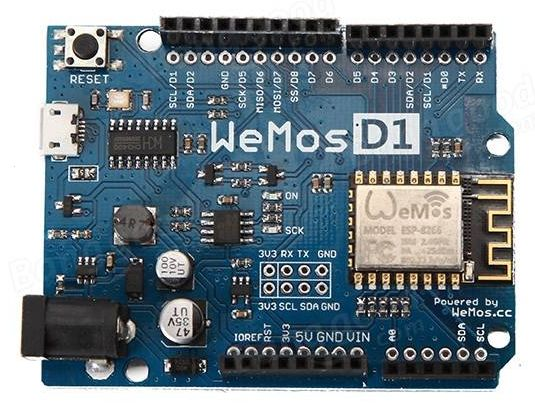
\includegraphics[scale=.5]{esp8266-wemos-d1}}
            \end{center}
            \caption{Module ESP8266 Wemos D1}
            \label{Fig:esp8266-wemos-d1}
        \end{figure}

    Sử dụng cổng Micro USB kết nối module với máy tính để nạp chương trình cho module. Nguồn cấp cho module ESP8266 Wemos D1 hoạt động là 5VDC.

    Quan sát bên ngoài phần cứng, module ESP8266 Wemos D1 có 11 chân dùng để xử lý tín hiệu digital và 1 chân dùng để xử lý tín hiệu analog.

    Module ESP8266 Wemos D1 cho phép sử dụng trực tiếp phần mềm lập trình Arduino IDE để viết chương trình và nạp chương trình cho nó với một số cài đặt cần thiết trong Arduino IDE.
\subsection{Lập trình với module ESP8266 Wemos D1}
    \begin{itemize}
        \item Phần cứng:
            \begin{itemize}
                \item Module ESP8266 Wemos D1.
                \item Cáp Micro USB dùng để nạp chương trình.
                \item Nguồn 5VDC cấp cho module ESP8266 Wemos D1 hoạt động.
                \item Các phần cứng khác tùy vào ứng dụng cụ thể.
            \end{itemize}

        \item Phần mềm:
            \begin{itemize}
                \item Phần mềm lập trình Arduino IDE (arduino.cc/en/Main/Software).
                \item Driver cài đặt cho cáp Micro USB.
            \end{itemize}

        \item Gọi tên các chân GPIO khi lập trình:
            \begin{itemize}
                \item Gọi theo các tên ký hiệu trên module, ví dụ: D0, D1,\ldots\, A0 (trên \fig{\ref{Fig:esp8266-wemos-d1}}).
                \item Gọi tên chân theo tên GPIO: được ghi trong \fig{\ref{Fig:chuc-nang-pin-esp8266-wemos-d1}}.
                \item Một số chân thực hiện được đa chức năng như Interrupt/PWM/I2C/1-Wire,\ldots\ được mô tả trên \fig{\ref{Fig:chuc-nang-pin-esp8266-wemos-d1}}. Với chân analog A0 tín hiệu đưa vào tối đa là 3.3V, module ESP8266 Wemos D1 chỉ hỗ trợ một chân xử lý tín hiệu analog.
                    \begin{figure}[!hp]
                        \begin{center}
                            \fbox{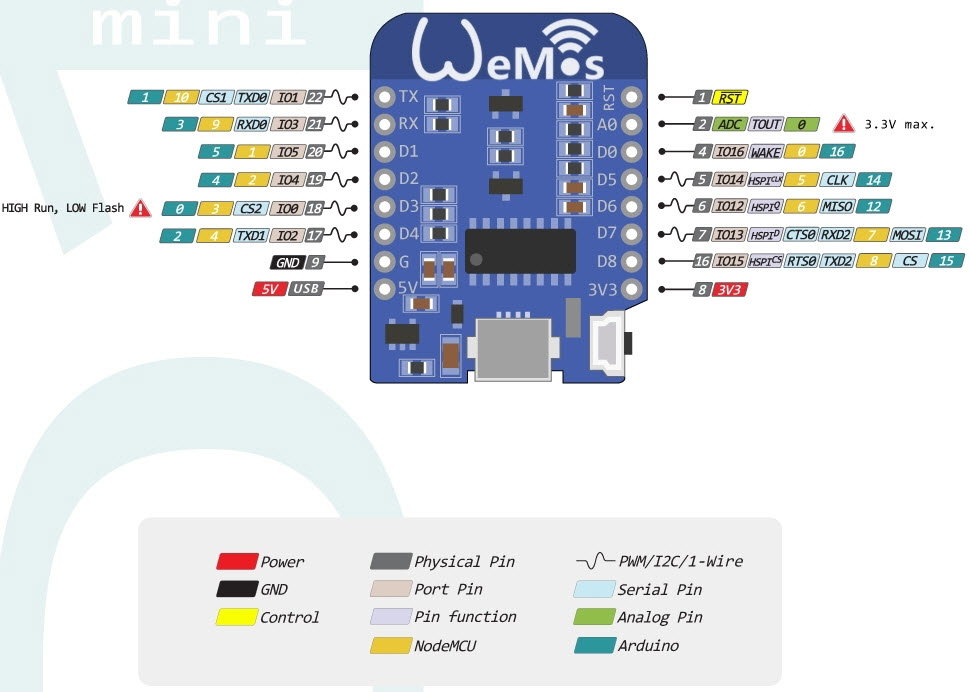
\includegraphics[scale=.6]{d1-mini-esp8266-pinout.jpg}}
                        \end{center}
                        \caption{Chức năng của các chân trên module ESP8266 Wemos D1 (Mini)} \label{Fig:chuc-nang-pin-esp8266-wemos-d1}
                    \end{figure}
            \end{itemize}
    \end{itemize}

\section{Công cụ và ngôn ngữ lập trình cho Module ESP8266}
    \begin{itemize}
        \item Công cụ lập trình: sử dụng Arduino IDE với cấu hình cần thiết.
        \item Ngôn ngữ lập trình: sử dụng ngôn ngữ lập trình Arduino.
    \end{itemize}
\subsection{Cài đặt môi trường lập trình Arduino IDE}
    Truy cập vào địa chỉ https://www.arduino.cc/en/Main/Software để tải phần mềm về sử dụng trên máy tính. Sau khi lựa chọn phiên bản cài đặt phù hợp, chọn JUST DOWNLOAD để tiến hành tải về máy.
\subsection{Cài đặt môi trường lập trình cho ESP8266 trên Arduino IDE}
    Để sử dụng môi trường lập trình Arduino IDE lập trình cho module ESP8266, cần thiết lập theo các bước sau:
        \begin{itemize}
            \item Mở Arduino IDE, chọn File/Preferences được giao diện như \fig{\ref{Fig:Preferences-2-Arduino-IDE}}.
                \begin{figure}[htp]
                    \begin{center}
                        \subfloat[Tab Preferences \label{Fig:Preferences-2-Arduino-IDE}]
                            {
                                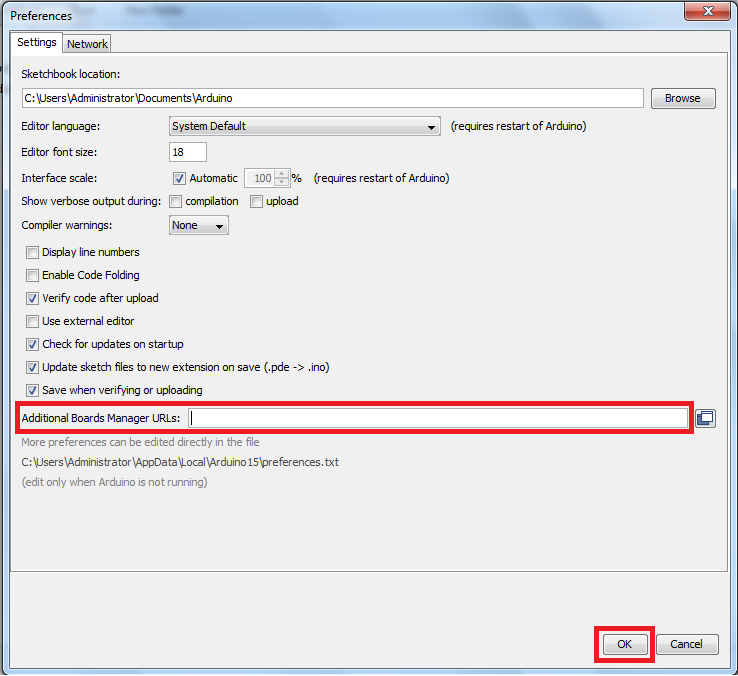
\includegraphics[scale=.35]{arduino-ide-preferences-2.png}
                            }\hspace{.5cm}
                        \subfloat[Điền URLs vào Additional Boards Manager URLs \label{Fig:Preferences-3-Arduino-IDE}]
                            {
                                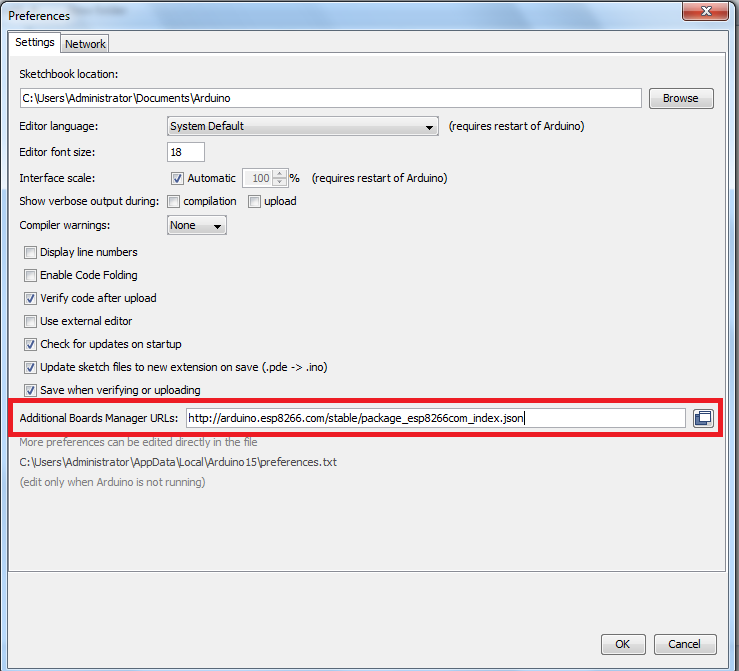
\includegraphics[scale=.35]{arduino-ide-preferences-3.png}
                            }
                    \end{center}
                    \caption{Arduino IDE Preferences}\label{Fig:Preferences-Arduino-IDE}
                \end{figure}
            \item Điền địa chỉ sau vào khung Additional Boards Manager URLs (\fig{\ref{Fig:Preferences-3-Arduino-IDE}}) và chọn OK: http://arduino.esp8266.com/stable/package\_esp8266com\_index.json
            \item Chọn Tool/Board/Boards Manager... Nhập từ khóa esp8266 vào khung tìm kiếm, chọn ESP8266 by ESP8266 Community và nhấn Install để cài đặt. Cài đặt hoàn thành chọn Close (\fig{\ref{Fig:Boards-Manager-Arduino-IDE}}).
                \begin{figure}[htp]
                    \begin{center}
                        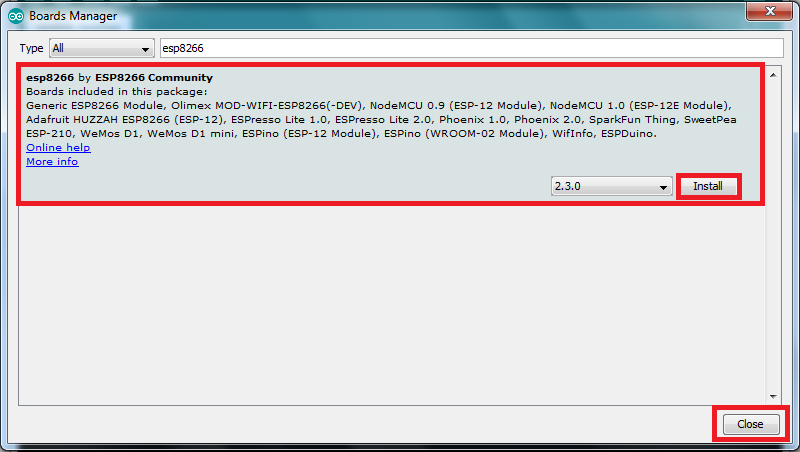
\includegraphics[scale=.58]{arduino-ide-boards-manager-2.png}
                    \end{center}
                    \caption{Arduino IDE Boards Manager -- ESP8266} \label{Fig:Boards-Manager-Arduino-IDE}
                \end{figure}
            \item Chọn Board để nạp chương trình cho ESP8266. Vào Tools, thiết lập các tùy chọn như sau:
                \begin{itemize}
                    \item Board: "WeMos D1 (Retried)".
                    \item CPU Frequency: "80 MHz".
                    \item Flash Size: "4M (3M SPIFFS)".
                    \item Upload Speed: "115200".
                    \item Port: "COM5" (thay đổi tên cổng COM cho phù hợp với từng máy tính).
                    \item Programer AVRISP mkII.
                \end{itemize}
        \end{itemize}

\section{Giao thức SmartConfig kết nối WiFi cho Module ESP8266}
\subsection{Giới thiệu giao thức SmartConfig}
    SmartConfig là một khái niệm được nhắc đến khi muốn cấu hình thông tin cho thiết bị WiFi kết nối nhanh chóng đến Internet nhất từ người dùng bằng chính thiết bị (điện thoại) của họ.

    SmartConfig có thể hiểu là chúng ta gửi thông tin mạng WiFi (bao gồm tên WiFi và password WiFi) cho ESP thông qua smartphone thay cho cách thông thường là phải khai báo thông tin này trong chương trình và nạp firmware xuống.

    SmartConfig có một số lợi ích sau:
        \begin{itemize}
            \item Dễ dàng cấu hình WiFi cho ESP8266 thông qua smartphone.
            \item Không cần phải nạp lại code để cấu hình.
            \item Có thể dùng SmartConfig để cấu hình nhiều thiết bị cùng một lúc.
        \end{itemize}
\subsection{Một số ứng dụng trên điện thoại để thực hiện SmartConfig}
    \begin{itemize}
        \item Sử dụng App ESP Touch (trên iOS) hoặc App ESP SmartConfig (trên Android) để thực hiện kết nối WiFi qua giao thức SmartConfig cho ESP8266.

        \item Ví dụ về cách hoạt động của giao thức ESP Touch gửi thông tin của mạng WiFi cho ESP8266: ESP Touch là protocol được dùng trong SmartConfig để người dùng có thể kết nối tới các phiên bản module ESP8266 thông qua cấu hình đơn giản trên Smartphone. Ban đầu không thể kết nối với ESP8266, nhưng thông qua giao thức ESP TOUCH thì Smartphone sẽ gửi gói UDP tới Access Point (AP) ở đây là ESP8266, mã hóa SSID và mật khẩu thành trường Length trong gói UDP, để ESP8266 có thể hiểu và giải mã được thông tin.
    \end{itemize}
\subsection{Sử dụng App ESP Touch trên iOS thực hiện SmartConfig cho ESP8266}
    \begin{itemize}
        \item Cài đặt App Esptouch cho điện thoại (trên hệ điều hành iOS).
        \item Cách thực hiện kết nối WiFi cho ESP8266 thông qua SmartConfig với App Esptouch:
            \begin{itemize}
                \item Mở App Esptouch (\fig{\ref{Fig:esptouch-1}}), nhập mật khẩu WiFi mà điện thoại đang kết nối vào (\fig{\ref{Fig:esptouch-2}}).
                \item Nhấn Confirm để gửi thông tin của mạng WiFi cho ESP8266 và đợi phản hồi về: nếu kết quả giống \fig{\ref{Fig:esptouch-3}} là ESP8266 kết nối WiFi thành công.
            \end{itemize}
            \begin{figure}[htp]
                \begin{center}
                    \subfloat[Mở App Esptouch \label{Fig:esptouch-1}]
                        {
                            \fbox{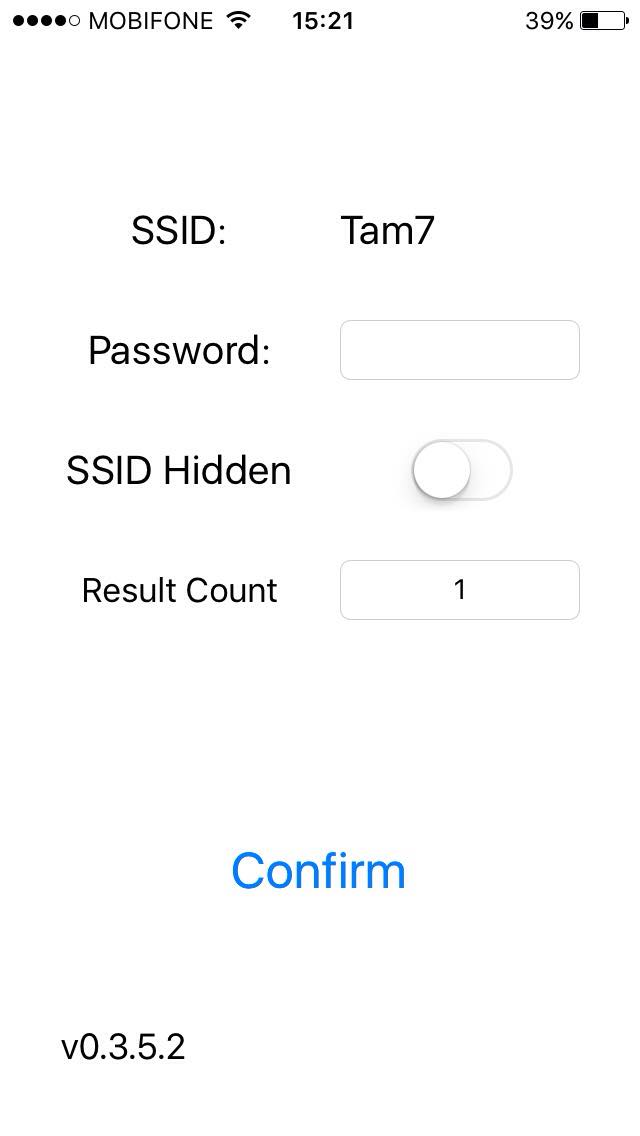
\includegraphics[scale=.2]{esptouch-1}}
                        }
                    \subfloat[Nhập password của mạng WiFi \label{Fig:esptouch-2}]
                        {
                            \fbox{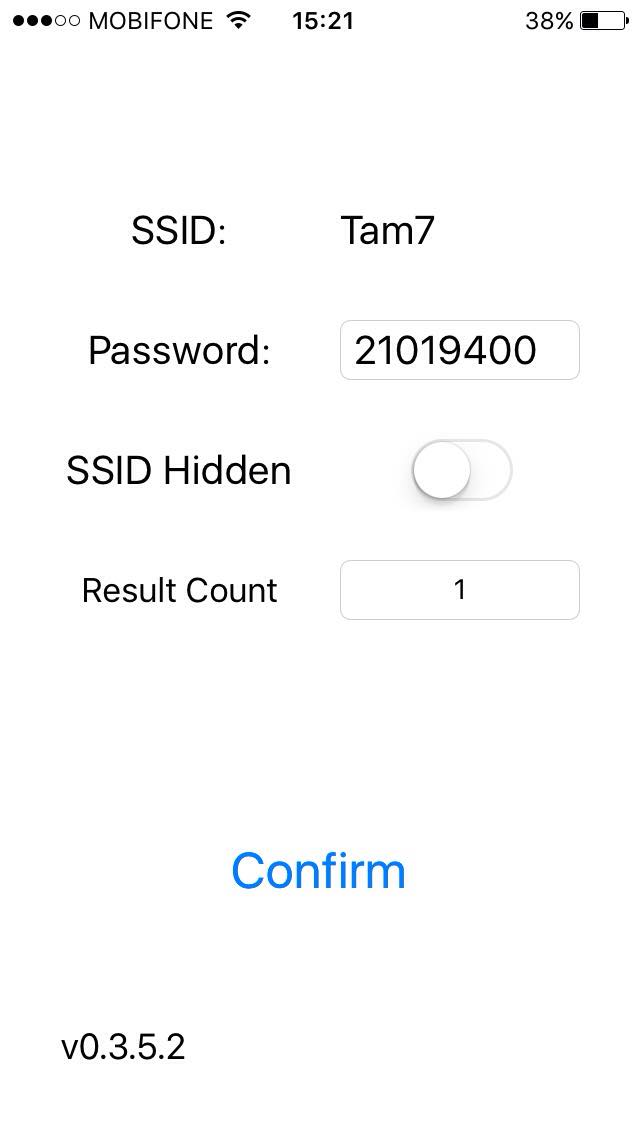
\includegraphics[scale=.2]{esptouch-2}}
                        }
                    \subfloat[Kết nối thành công \label{Fig:esptouch-3}]
                        {
                            \fbox{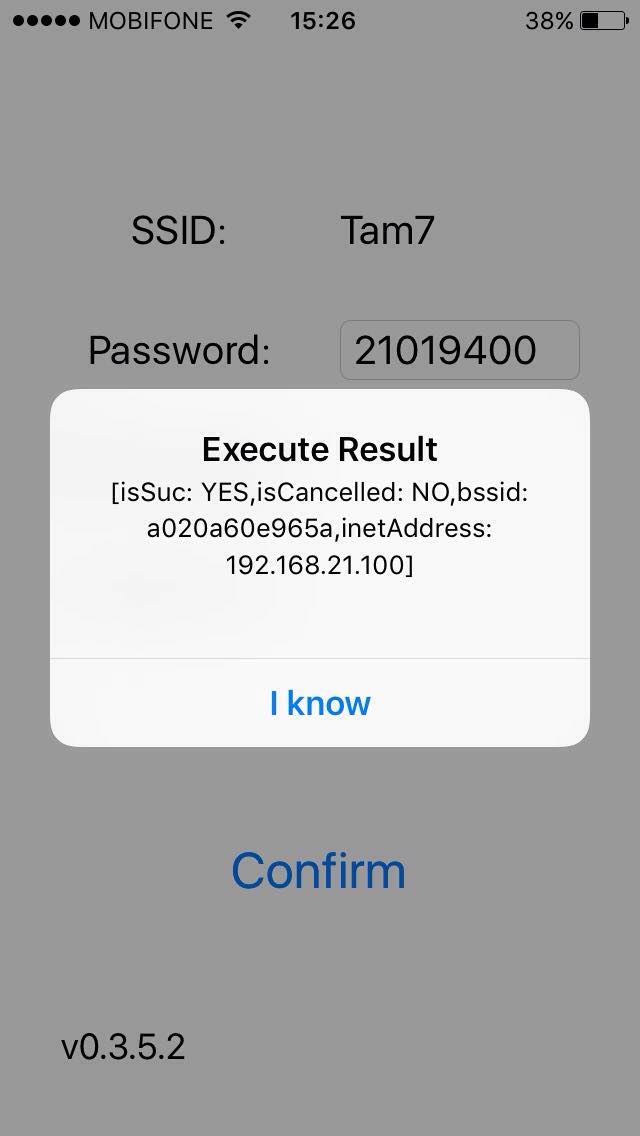
\includegraphics[scale=.2]{esptouch-3}}
                        }
                \end{center}
                \caption{Thực hiện SmartConfig với App Esptouch trên iOS}\label{Fig:smartconfig-esptouch}
            \end{figure}
    \end{itemize}

\newpage
\section{Ứng dụng Blynk trên điện thoại}
\subsection{Giới thiệu}
	Blynk là ứng dụng điện thoại trên hệ điều hành iOS và Android hỗ trợ viết các ứng dụng di động cho các thiết bị thông minh. Ứng dụng cho phép chúng ta dễ dàng kết nối với các mạch tích hợp thông dụng như Arduino, Raspberry Pi, ESP8266, Particle (Photon/SparkCore) và điều khiển thông qua Internet.
\subsection{Cài đặt App Blynk và thư viện Bkynk cho lập trình}
    \begin{itemize}
        \item Tải App Blynk về cài đặt trên điện thoại.
        \item Mở App Blynk và tạo tài khoản sử dụng App.
        \item Tải thư viện Blynk hỗ trợ viết chương trình: github.com/blynkkk/blynk-library
    \end{itemize}
\subsection{Tạo project trong App Blynk}
    Các thuộc tính cần lưu ý: Choose Device (vi điều khiển đang sử dụng), Connection Type (hình thức kết nối để điều khiển, ví dụ là WiFi) và Auth Token (mã xác thực kết nối giữa vi điều khiển và App Blynk).
        \begin{figure}[!ht]
            \begin{center}
                \subfloat[Chọn New Project \label{Fig:blynk-create-project-1}]
                    {
                        \fbox{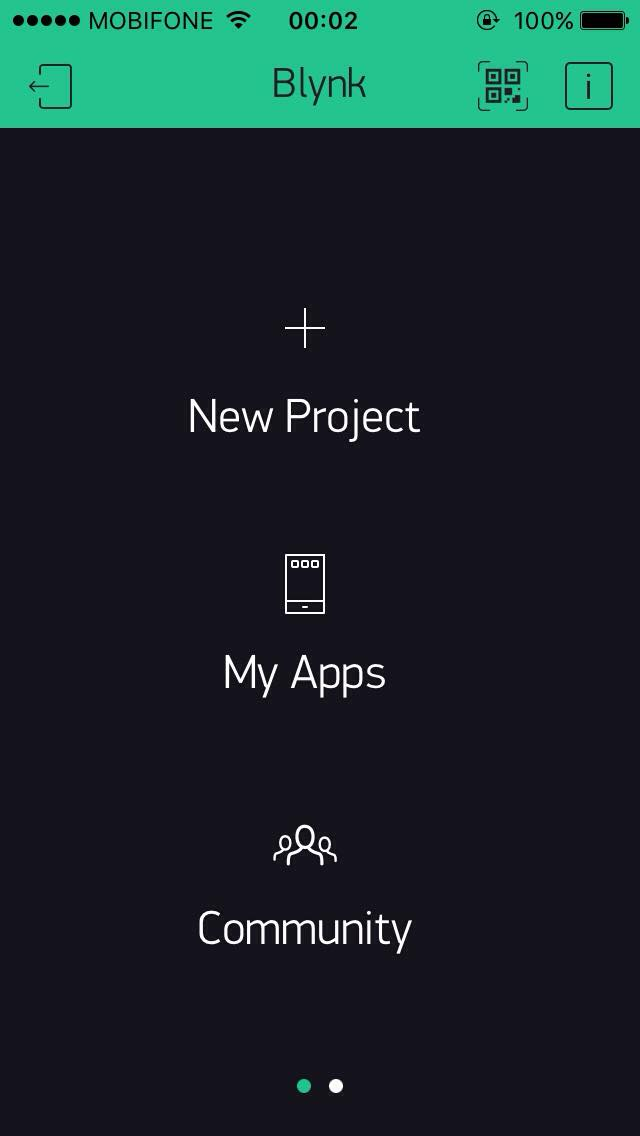
\includegraphics[scale=.2]{create-project-1}}
                    }
                \subfloat[Thay đổi thông tin project \label{Fig:blynk-create-project-2}]
                    {
                        \fbox{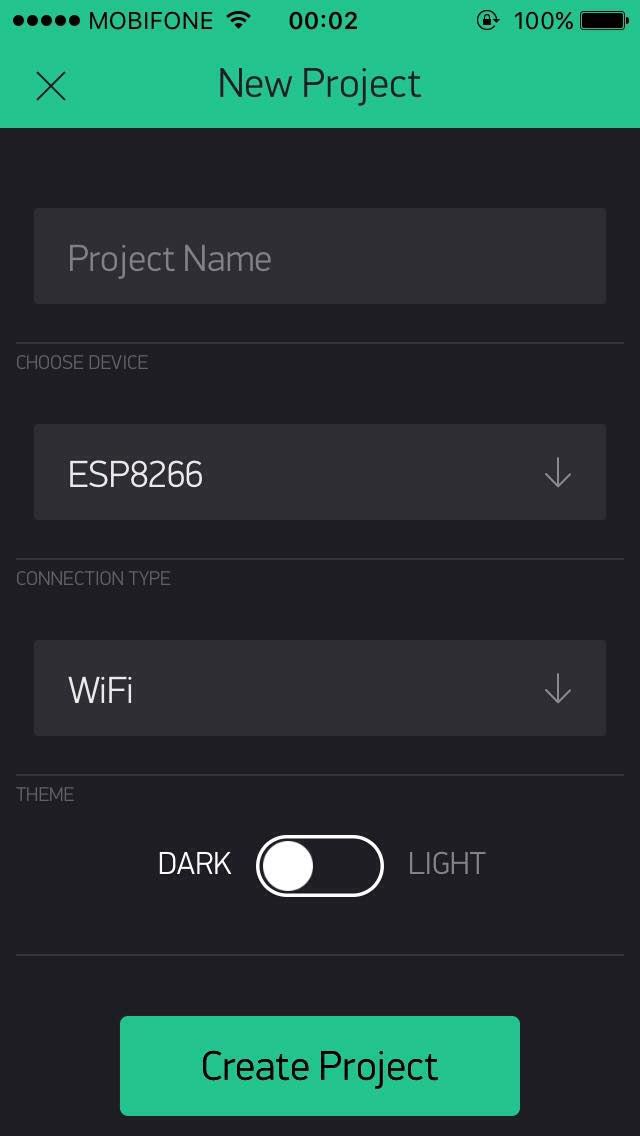
\includegraphics[scale=.2]{create-project-2}}
                    }
                \subfloat[Thông tin project \label{Fig:blynk-create-project-3}]
                    {
                        \fbox{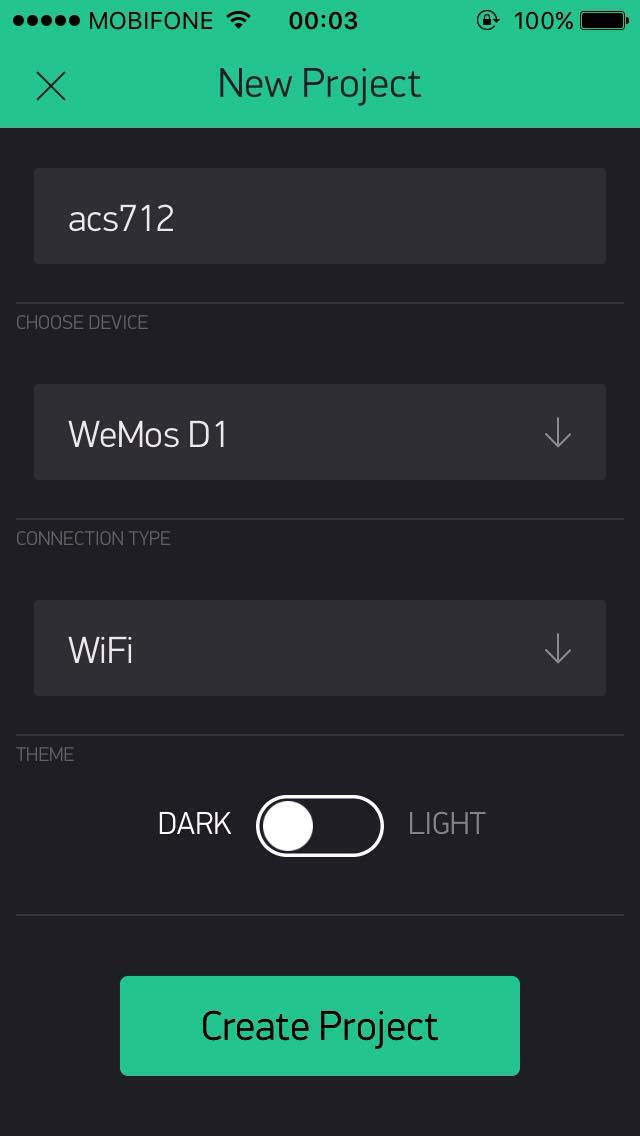
\includegraphics[scale=.2]{create-project-3}}
                    }\\
                \subfloat[Giao diện thiết kế \label{Fig:blynk-create-project-4}]
                    {
                        \fbox{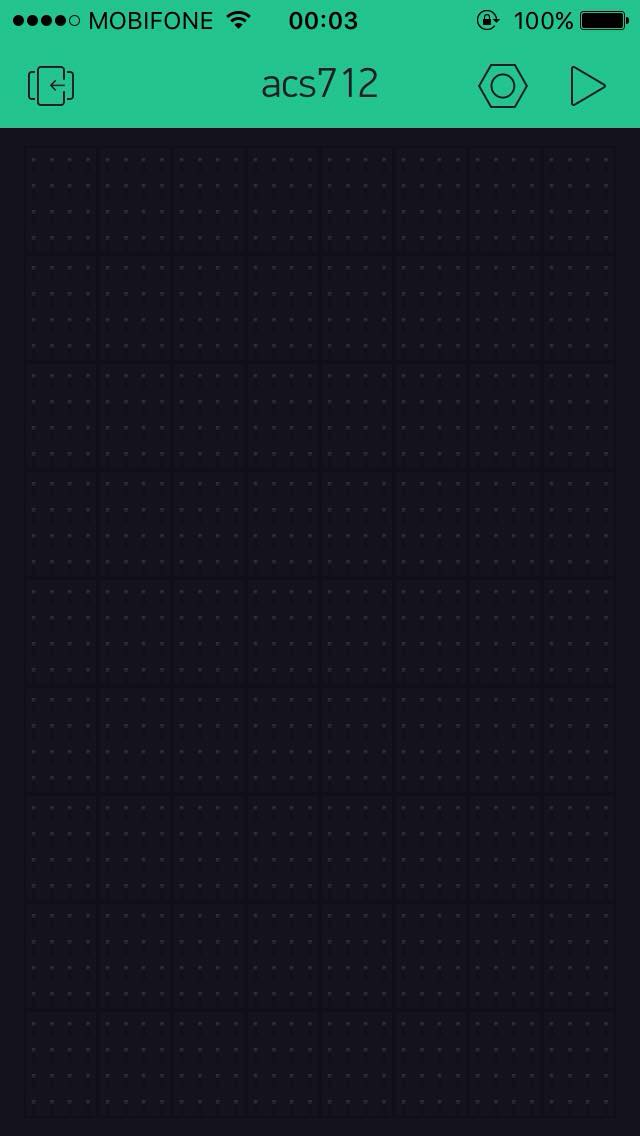
\includegraphics[scale=.2]{create-project-4}}
                    }
                \subfloat[Auth Token của project\label{Fig:blynk-create-project-5}]
                    {
                        \fbox{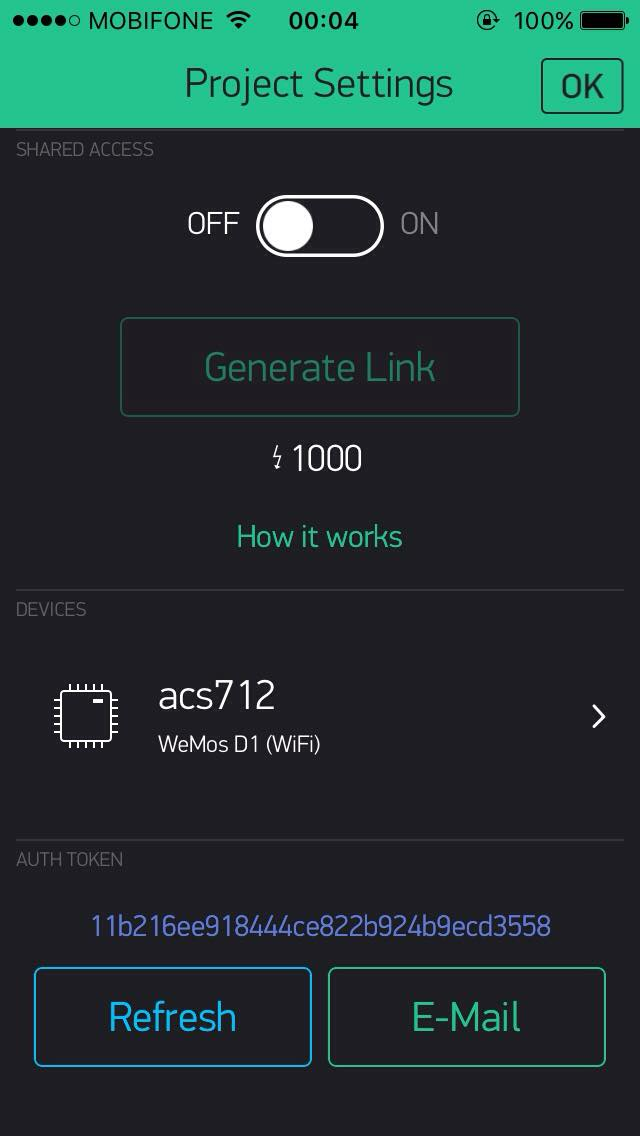
\includegraphics[scale=.2]{create-project-5}}
                    }
            \end{center}
            \caption{Tạo project trong App Blynk}\label{Fig:app-blynk-project}
            % \vspace{-2cm}
        \end{figure}
\subsection{Kết nối giữa các phần tử trên App Blynk và vi điều khiển}
    \begin{itemize}
        \item Để kết nối giữa App Blynk và vi điều khiển: cần chọn đúng Device, Connection Type và lấy Auth Token (được gửi qua Email đăng ký tài khoản).
        \item Để kết nối các phần tử điều khiển trên App Blynk với vi điều khiển: cần biết chính xác PIN (Analog, Digital, Virtual) của các phần tử trên App Blynk để viết chương trình điều khiển tương ứng.
            \begin{itemize}
                \item Các PIN Analog và Digital thường dùng để điều khiển trực tiếp các phần cứng kết nối với vi điều khiển.
                \item Các PIN Vitual để tạo phần cứng ảo hỗ trợ cho vi điều khiển: điều khiển, hiển thị, truyền nhận dữ liệu giữa App và vi điều khiển.
            \end{itemize}
    \end{itemize}

\section{Ứng dụng Web Server Thingspeak}
\subsection{Giới thiệu}
    ThingSpeak là mã nguồn mở cho các ứng dụng Internet of Things -- IoT, hỗ trợ các API lữu trữ, lấy dữ liệu từ thiết bị sử dụng HTTP thông qua kết nối Internet.
\subsection{Cài đặt thư viện Thingspeak cho lập trình}
    Tải thư viện Thingspeak hỗ trợ viết chương trình: github.com/mathworks/thingspeak-arduino
\subsection{Tạo tài khoản sử dụng và tạo project trên Thingspeak}
    \begin{figure}[htp]
        \begin{center}
            \fbox{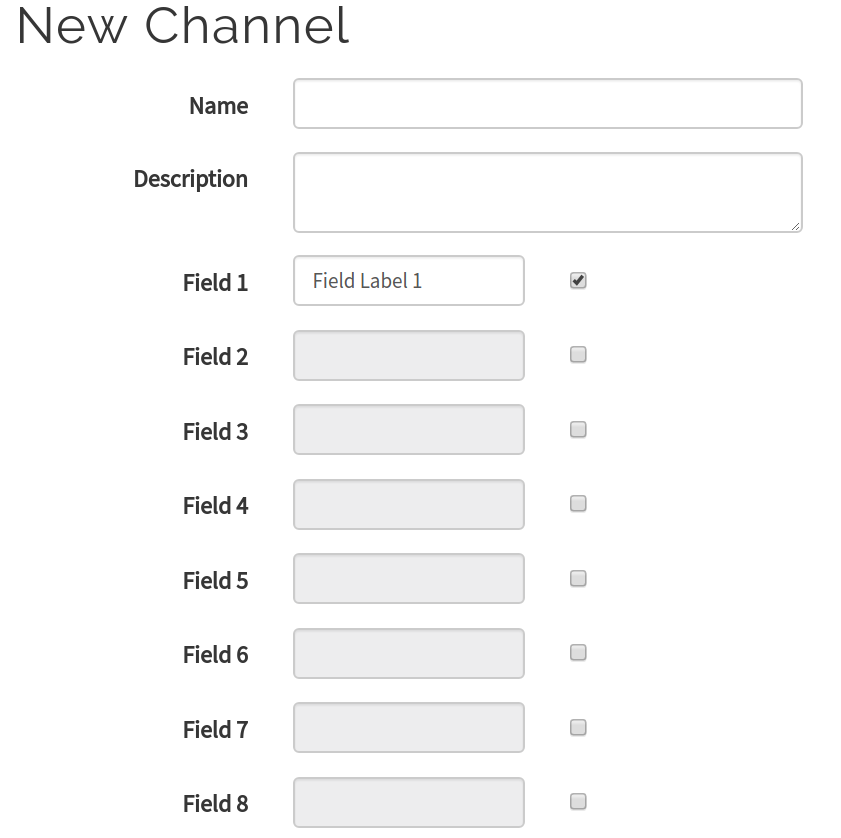
\includegraphics[scale=.3]{create-project}}
        \end{center}
        \caption{Các Field dùng lưu trữ dữ liệu trên Thingspeak} \label{Fig:thingspeak-create-project}
    \end{figure}
    \begin{itemize}
        \item Truy cập vào địa chỉ thingspeak.com, tạo tài khoản sử dụng Thingspeak.
        \item Chọn New Channel để tạo project mới: đặt tên cho project, thông tin mô tả cho project, tên cho các Field và chọn Save Channel. Các Field 1 đến Field 8 là các field dùng để lưu trữ dữ liệu từ vi điều khiển gửi lên Thingspeak (\fig{\ref{Fig:thingspeak-create-project}}).
        \item Để kết nối giữa Web Server Thingspeak và vi điều khiển cần có Channel ID và Write API Key (vào tab API Keys để lấy Write API Key).
    \end{itemize}
\subsection{Cách giao tiếp vi điều khiển và Web Server Thingspeak}
    Sử dụng phương thức POST/GET/\ldots trong giao thức HTTP để gửi dữ liệu lên Web Server Thingspeak.

\section{Cảm biến dòng điện ACS712}
\subsection{Giới thiệu}
    Cảm biến dòng điện ACS712 là IC cảm biến dòng tuyến tính dựa trên hiệu ứng Hall. Cảm biến xuất ra tín hiệu analog Vout biến đổi tuyến tính theo sự thay đổi của dòng điện được lấy mẫu thứ cấp DC (hoặc AC), trong phạm vi đã cho. Tụ (Cf theo sơ đồ) được dùng với mục đích chống nhiễu và có giá trị tùy thuộc vào từng mục đích sử dụng.
        \begin{figure}[htp]
            \begin{center}
                \subfloat[]
                    {
                        \fbox{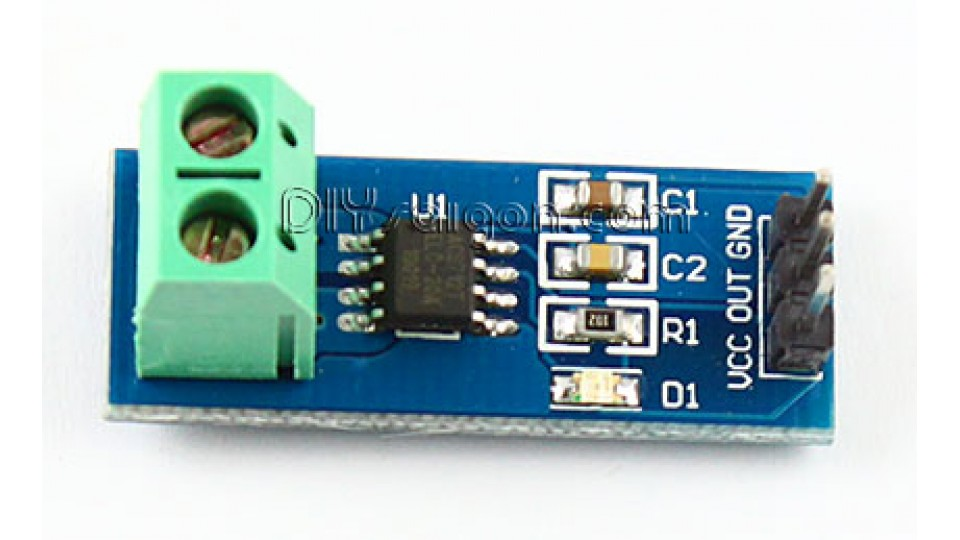
\includegraphics[scale=.28]{acs712}}
                    }
                \subfloat[]
                    {
                        \fbox{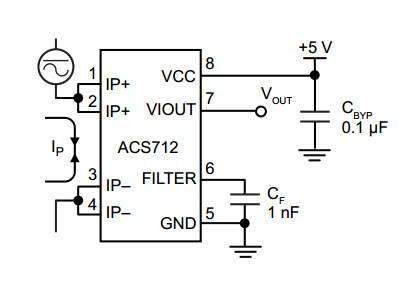
\includegraphics[scale=.5]{acs712-schem}}
                    }
            \end{center}
            \caption{Cảm biến dòng ACS712} \label{Fig:acs712}
        \end{figure}
\subsection{Đặc điểm của cảm biến}
    \begin{itemize}
        \item Thời gian tăng của đầu ra để đáp ứng với đầu vào là 5$\mu$s.
        \item Điện trở dây dẫn trong là 1.2m$\Omega$.
        \item Điện áp hoạt động 5V.
        \item Độ nhạy đầu ra từ 63 -- 190mV/A ứng với từng loại cảm biến: 64 -- 68 mV/A (loại 30A); 96 -- 104mV/A (loại 20A) và 180 -- 190mV/A (loại 5A).
        \item Điện áp ra ổn định.
    \end{itemize}
\subsection{Cách sử dụng module cảm biến dòng ACS712}
    \begin{itemize}
        \item Đo dòng điện DC:
            \begin{itemize}
                \item Khi đo DC phải mắc tải nối tiếp $Ip+$ và $Ip-$ đúng chiều, dòng điện đi từ $Ip+$ đến $Ip-$ để Vout ra mức điện thế 2.5V đến 5V tương ứng dòng 0 đến $I_{\textrm{đmcb}}$ (dòng điện định mức mà cảm biến đo được), nếu mắc ngược Vout sẽ ra điện thế 2.5V đến 0V tương ứng với 0A đến $-I_{\textrm{đmcb}}$.
                \item Cấp nguồn 5V cho module khi chưa có dòng $Ip$ (chưa có tải mắc nối tiếp với domino), thì Vout là 2.5V. Khi dòng $Ip$ (dòng của tải) bằng $I_{\textrm{đmcb}}$ thì Vout là 5V, Vout sẽ tuyến tính với dòng $Ip$, trong khoảng 2.5V đến 5V tương ứng với dòng 0 đến $I_{\textrm{đmcb}}$.
                \item Công thức tính dòng điện DC (với $V_m$ là độ nhạy ứng với từng loại cảm biến dòng ACS712 được trình bày ở trên):
                    \begin{align*}
                        V_{(mV)} = \dfrac{adc \times 5000.0}{1024.0};\quad I_{(mA)} = \dfrac{V - 2500}{V_m} \quad \textrm{(với } V_m \textrm{ là độ nhạy)}
                    \end{align*}
            \end{itemize}

        \item Đo dòng điện AC:
            \begin{itemize}
                \item Khi đo dòng điện AC, do dòng điện AC không có chiều nên không cần quan tâm chiều.
                \item Cấp nguồn 5V cho module khi chưa có dòng $Ip$ (chưa có tải mắc nối tiếp với domino), thì Vout là 2.5V. khi có dòng xoay chiều $Ip$ (dòng AC) do dòng xoay chiều độ lớn thay đổi liên tục theo hàm sin, nên điện thế Vout sẽ là điện thế xoay chiều hình sin có độ lớn tuyến tính với dòng điện AC, 0 đến 5V (thế xoay chiều) tương ứng với $-I_{\textrm{đmcb}}$ đến $+I_{\textrm{đmcb}}$ (dòng xoay chiều).
                \item Công thức tính dòng điện AC (với $V_m$ là độ nhạy ứng với từng loại cảm biến dòng ACS712 được trình bày ở trên):
                    \begin{align*}
                        V_{(mV)} = \dfrac{adc_{MaxPoint} \times 5000.0}{1024.0};\quad I_{(mA)} = \dfrac{V - 2500}{\sqrt{2}V_m} \quad \textrm{(với } V_m \textrm{ là độ nhạy)}
                    \end{align*}
            \end{itemize}
    \end{itemize}

\section{Xác định công suất, điện năng tiêu thụ của phụ tải xoay chiều một pha dựa vào dòng điện qua tải và thời gian hoạt động của tải}
    \begin{itemize}
        \item Công suất tiêu thụ của phụ tải xoay chiều một pha: $P = UI\cos \varphi$.
        \item Giá trị dòng điện đo được là giá trị tức thời: $I_{i}$.
        \item Công suất tức thời: $P = U_iI_i\cos \varphi_i$
        \item Công suất trung bình có thể xác định gần đúng bằng công thức sau:
            \begin{align*}
                P_{tb} = \dfrac{1}{n}\sum^n_{i=1}P_i
            \end{align*}
        \item Do cảm biến ACS712 chỉ có thể được dòng điện đi qua phụ tải, không đo được điện áp cấp cho phụ tải. Để đơn giản chọn điện áp $U$ cấp cho phụ tải một pha và hệ số công suất $\cos \varphi$ là không đổi, khi đó ta có:
            \begin{align*}
                P_{tb} = \dfrac{1}{n}\sum^n_{i=1}P_i = \dfrac{U\cos \varphi}{n}\sum^n_{i=1}I_i
            \end{align*}
            Khi tính toán, có thể chọn gần đúng $U = 220V$ và $\cos \varphi = 0.86$
        \item Điện năng tiêu thụ của phụ tải: $A = \sum^m_{j=1} P_{tb_j}t_j$ với $P_{tb_j}$ là công suất trung bình trong thời gian phụ tải hoạt động $t_j$.
    \end{itemize}



    %----------------------------------------------------------------------------------------
    %    Chương 2 - Sơ đồ mạch và nguyên lý hoạt động
    %----------------------------------------------------------------------------------------
    \chapter{THIẾT KẾ MẠCH VÀ GIAO DIỆN ĐIỀU KHIỂN}

\section{Sơ đồ khối}
    Sơ đồ khối thiết kế bộ điều khiển được mô tả trên \fig{\ref{Fig:block-diagram}}:

    \begin{figure}[htp]
        \begin{center}
            %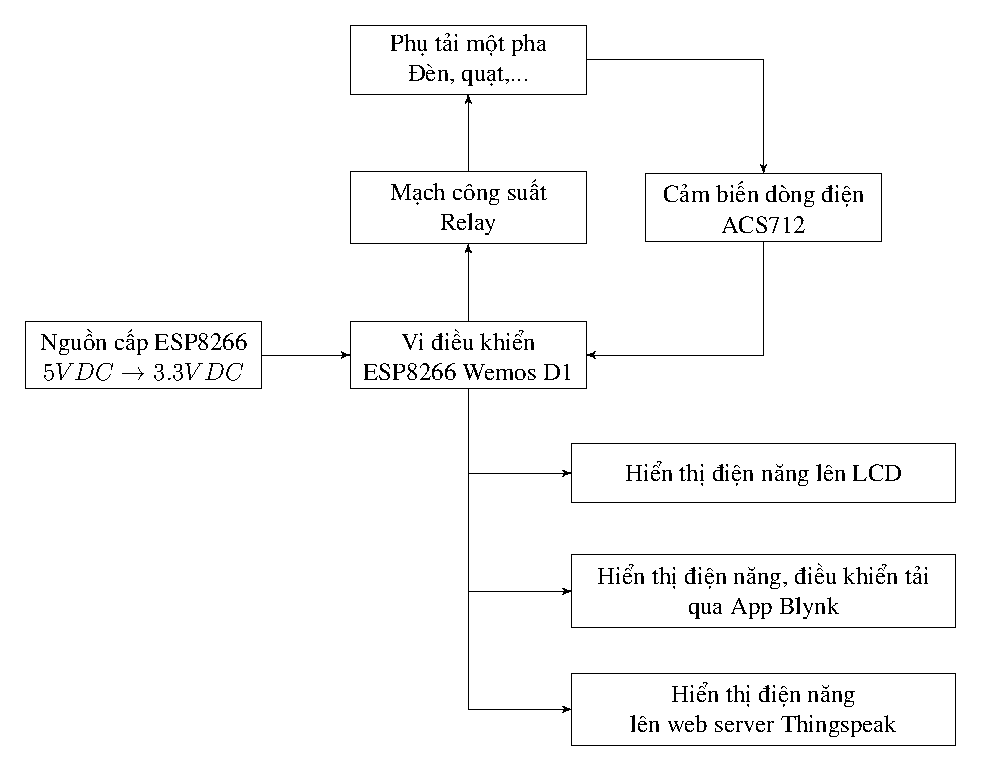
\includegraphics[scale=1]{block-diagram.pdf}
            \subimport{../flowchart/}{block-diagram.tex}
        \end{center}
        \caption{Sơ đồ khối thiết kế bộ điều khiển} \label{Fig:block-diagram}
    \end{figure}

    Mô tả các khối chức năng trên \fig{\ref{Fig:block-diagram}}:
    \begin{itemize}
        \item Sử dụng vi điều khiển ESP8266 Wemos D1 với khả năng giao tiếp WiFi (với nguồn hoạt động 5VDC $\rightarrow$ 3.3VDC).
        \item Điều khiển tải thông qua mạch công suất với Relay (sử dụng nguồn kích 5VDC).
        \item Sử dụng cảm biến dòng điện ACS712 để đo dòng điện tiêu thụ của phụ tải xoay chiều một pha, từ đó tính công suất, điện năng tiêu thụ của phụ tải.
        \item Hiển thị, gửi dữ liệu thu thập được (dòng điện, công suất) lên LCD (quan sát trực tiếp), App Blynk (quan sát trên thiết bị di động) và Server Thingspeak (quan sát trên Web).
    \end{itemize}

\section{Sơ đồ mạch nguyên lý}
    Sơ đồ mạch nguyên lý được mô tả trên \fig{\ref{Fig:powerACS712_schem}}:
        \begin{figure}[htp]
            \begin{center}
                \fbox{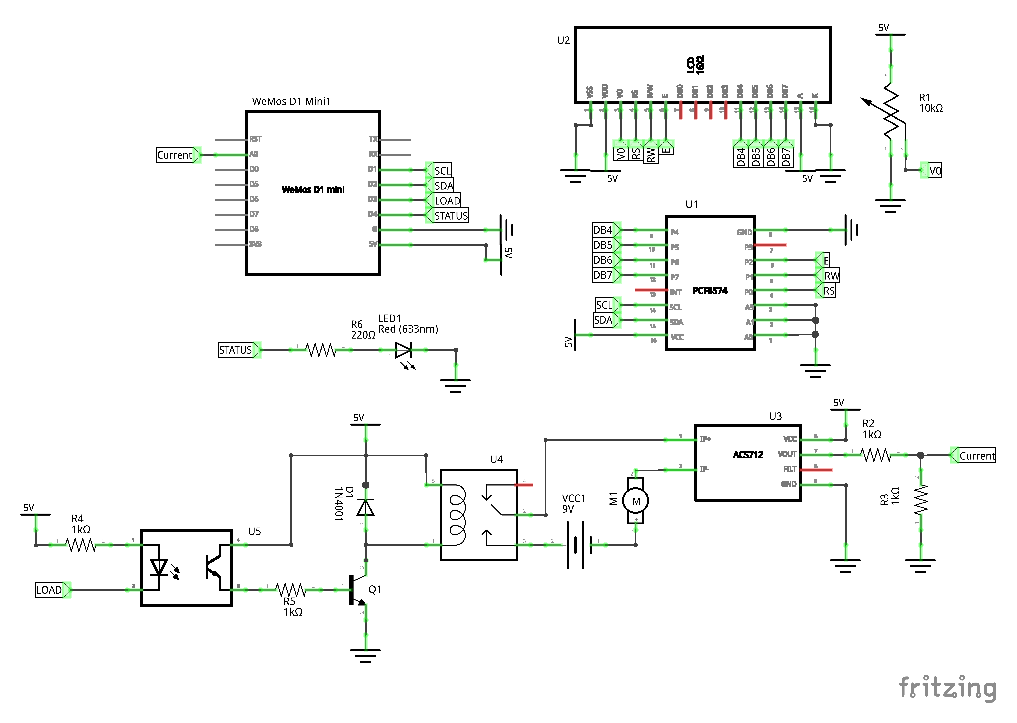
\includegraphics[scale=.85]{powerACS712_schem.pdf}}
            \end{center}
            \caption{Sơ đồ mạch nguyên lý} \label{Fig:powerACS712_schem}
        \end{figure}

\section{Mô tả các khối chức năng trên sơ đồ mạch nguyên lý}
    \begin{itemize}
        \item Hiển thị dòng điện và công suất với LCD 16x02 (sử dụng giao tiếp I2C).
        \item Đo dòng điện tiêu thụ của phụ tải với cảm biến dòng ACS712.
            \begin{itemize}
                \item Do tín hiệu điện áp đưa vào chân analog của ESP8266 Wemos D1 tối đa là 3.3V, trong khi đó tính hiệu trả về của cảm biến có thể lên đến 5.0V.
                \item Sử dụng cầu chia điện áp tại ngõ ra của cảm biến dòng để điện áp đưa vào chân analog của ESP8266 nhỏ hơn 3.3V. Do $R_2 = R_3 = R = 1 k \Omega$, nên:
                    \begin{align*}
                        V_o = \dfrac{R}{R + R} V_i = \dfrac{V_i}{2} \Longrightarrow V_i = 2.0 V_o
                    \end{align*}
                \item Khi đó các công thức tính dòng điện được xác định lại như sau:
                    \begin{itemize}
                        \item Với dòng DC:
                            \begin{align*}
                                V_{(mV)} & = \dfrac{2.0 \times adc \times 5000.0}{1024.0} = \dfrac{adc \times 5000.0}{521.0};\\ I_{(mA)} & = \dfrac{V - 2500}{V_m} \quad \textrm{(với } V_m \textrm{ là độ nhạy)}
                            \end{align*}
                        \item Với dòng AC:
                            \begin{align*}
                                V_{(mV)} & = \dfrac{2.0 \times adc_{MaxPoint} \times 5000.0}{1024.0} = \dfrac{adc_{MaxPoint} \times 5000.0}{512.0};\\ I_{(mA)} & = \dfrac{V - 2500}{\sqrt{2}V_m} \quad \textrm{(với } V_m \textrm{ là độ nhạy)}
                            \end{align*}
                    \end{itemize}
            \end{itemize}
        \item Điều khiển tải thông qua relay.
        \item LED báo trạng thái quá tải.
    \end{itemize}

\section{Giao diện điều khiển trên Blynk}
    \begin{figure}[htp]
        \begin{center}
            \fbox{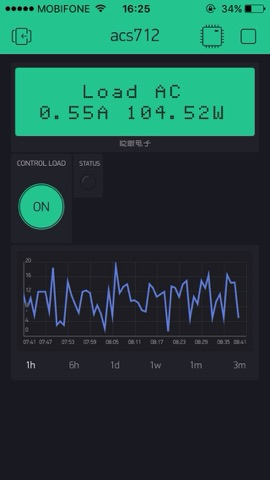
\includegraphics[scale=.5]{blynk-result}}
        \end{center}
        \caption{Giao diện điều khiển trên Blynk}
    \end{figure}

    \begin{table}[htp]
        \begin{center}
            \begin{tabular}{|l|c|l|} \hline
                \textbf{Phần tử} & \textbf{Pin} & \textbf{Giải thích} \\
                \hline
                LCD & V0 & Hiển thị dữ liệu \\
                \hline
                Button & D5 & Điều khiển tải \\
                \hline
                LED & V1 & Báo trạng thái quá tải \\
                \hline
                History Graph & V3/V4 & Dữ liệu dòng điện DC/AC\\
                \hline
            \end{tabular}
        \end{center}
        \caption{Các phần tử trên App Blynk}
    \end{table}

\newpage
\section{Giao diện thu thập dữ liệu trên Thingspeak}
    \begin{table}[htp]
        \begin{center}
            \begin{tabular}{|c|l|} \hline
                \textbf{Tên Field} & \textbf{Giải thích} \\
                \hline
                Field 3 & Dòng DC \\
                \hline
                Field 4 & Trạng thái quá tải \\
                \hline
                Field 5 & Công suất tiêu thụ \\
                \hline
            \end{tabular}
        \end{center}
        \caption{Các Field trên web Thingspeak}
    \end{table}



    %----------------------------------------------------------------------------------------
    %    Chương 3 - Lưu đồ giải thuật và chương trình
    %----------------------------------------------------------------------------------------
    \chapter{LƯU ĐỒ GIẢI THUẬT VÀ CHƯƠNG TRÌNH}

\section{Lưu đồ giải thuật}

    Lưu đồ giải thuật dùng cho chương trình được mô tả trên \fig{\ref{Fig:flowchart}}:

    \begin{figure}[htp]
        \begin{center}
            \hspace*{-1cm}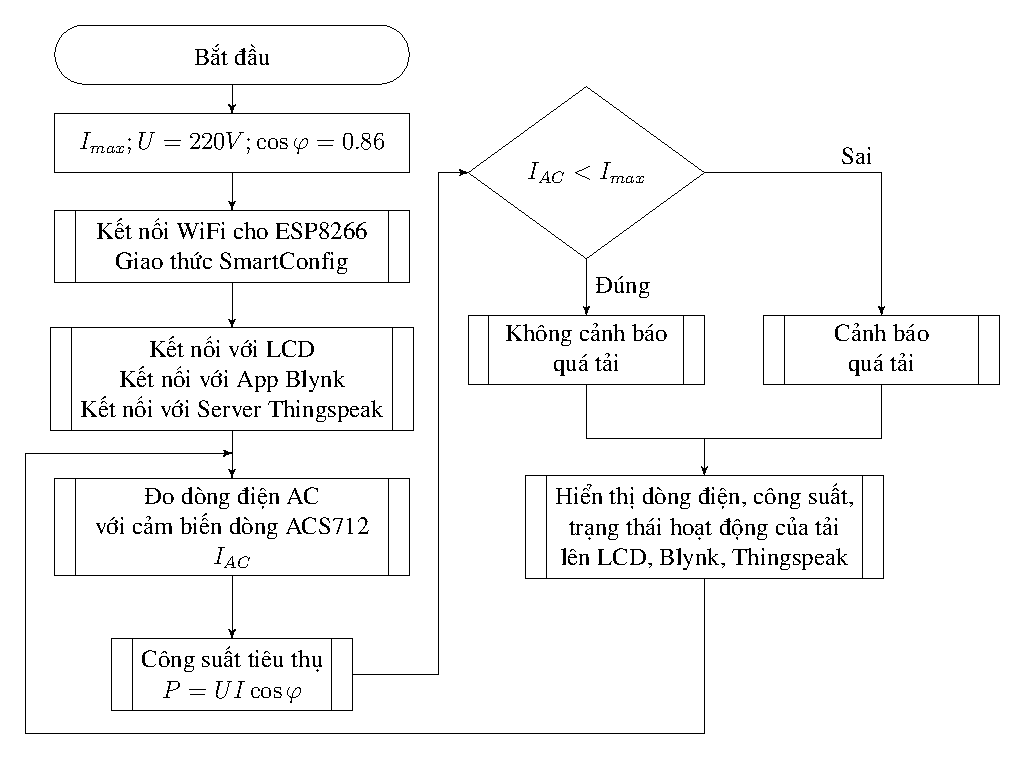
\includegraphics[scale=1]{flowchart.pdf}
            % \subimport{../flowchart/}{flowchart.tex}
        \end{center}
        \caption{Sơ đồ khối thiết kế bộ điều khiển} \label{Fig:flowchart}
    \end{figure}

\section{Chương trình điều khiển}
    \lstinputlisting{acs712_arduino.ino}

\section{Kết quả thu được}
    \begin{figure}[htp]
        \begin{center}
            \hspace*{-1cm}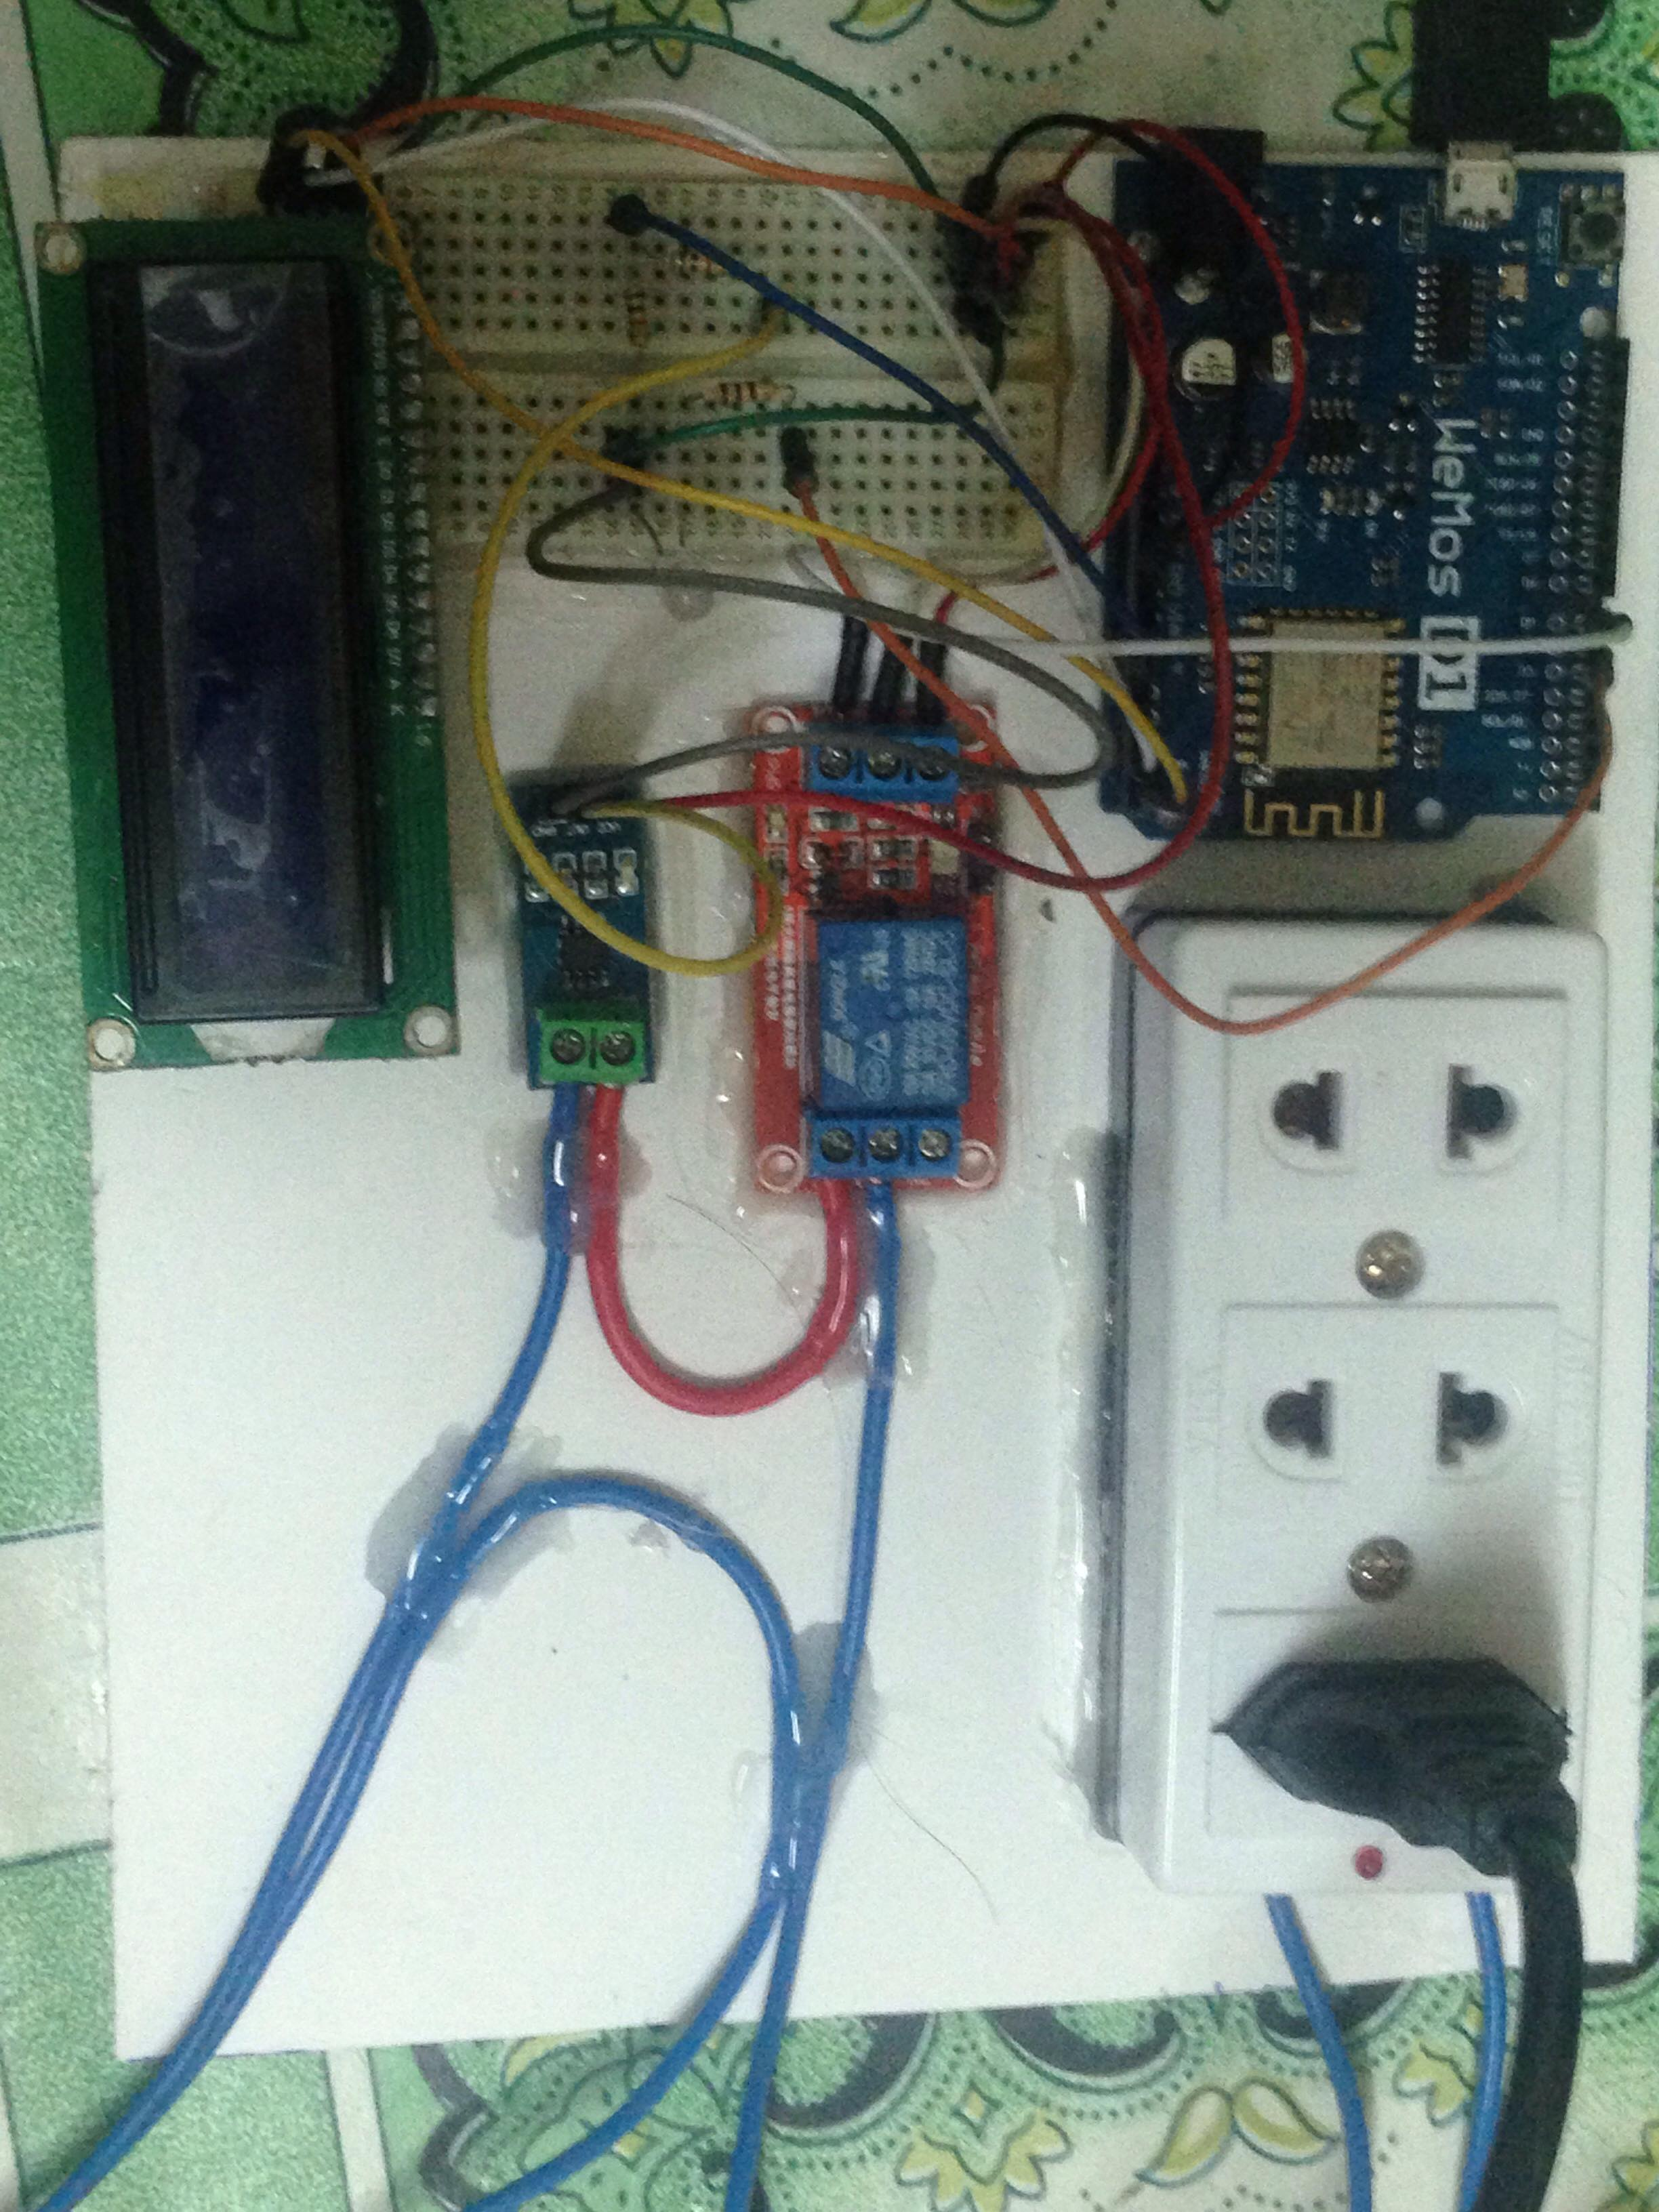
\includegraphics[scale=.08]{hardware-1}
            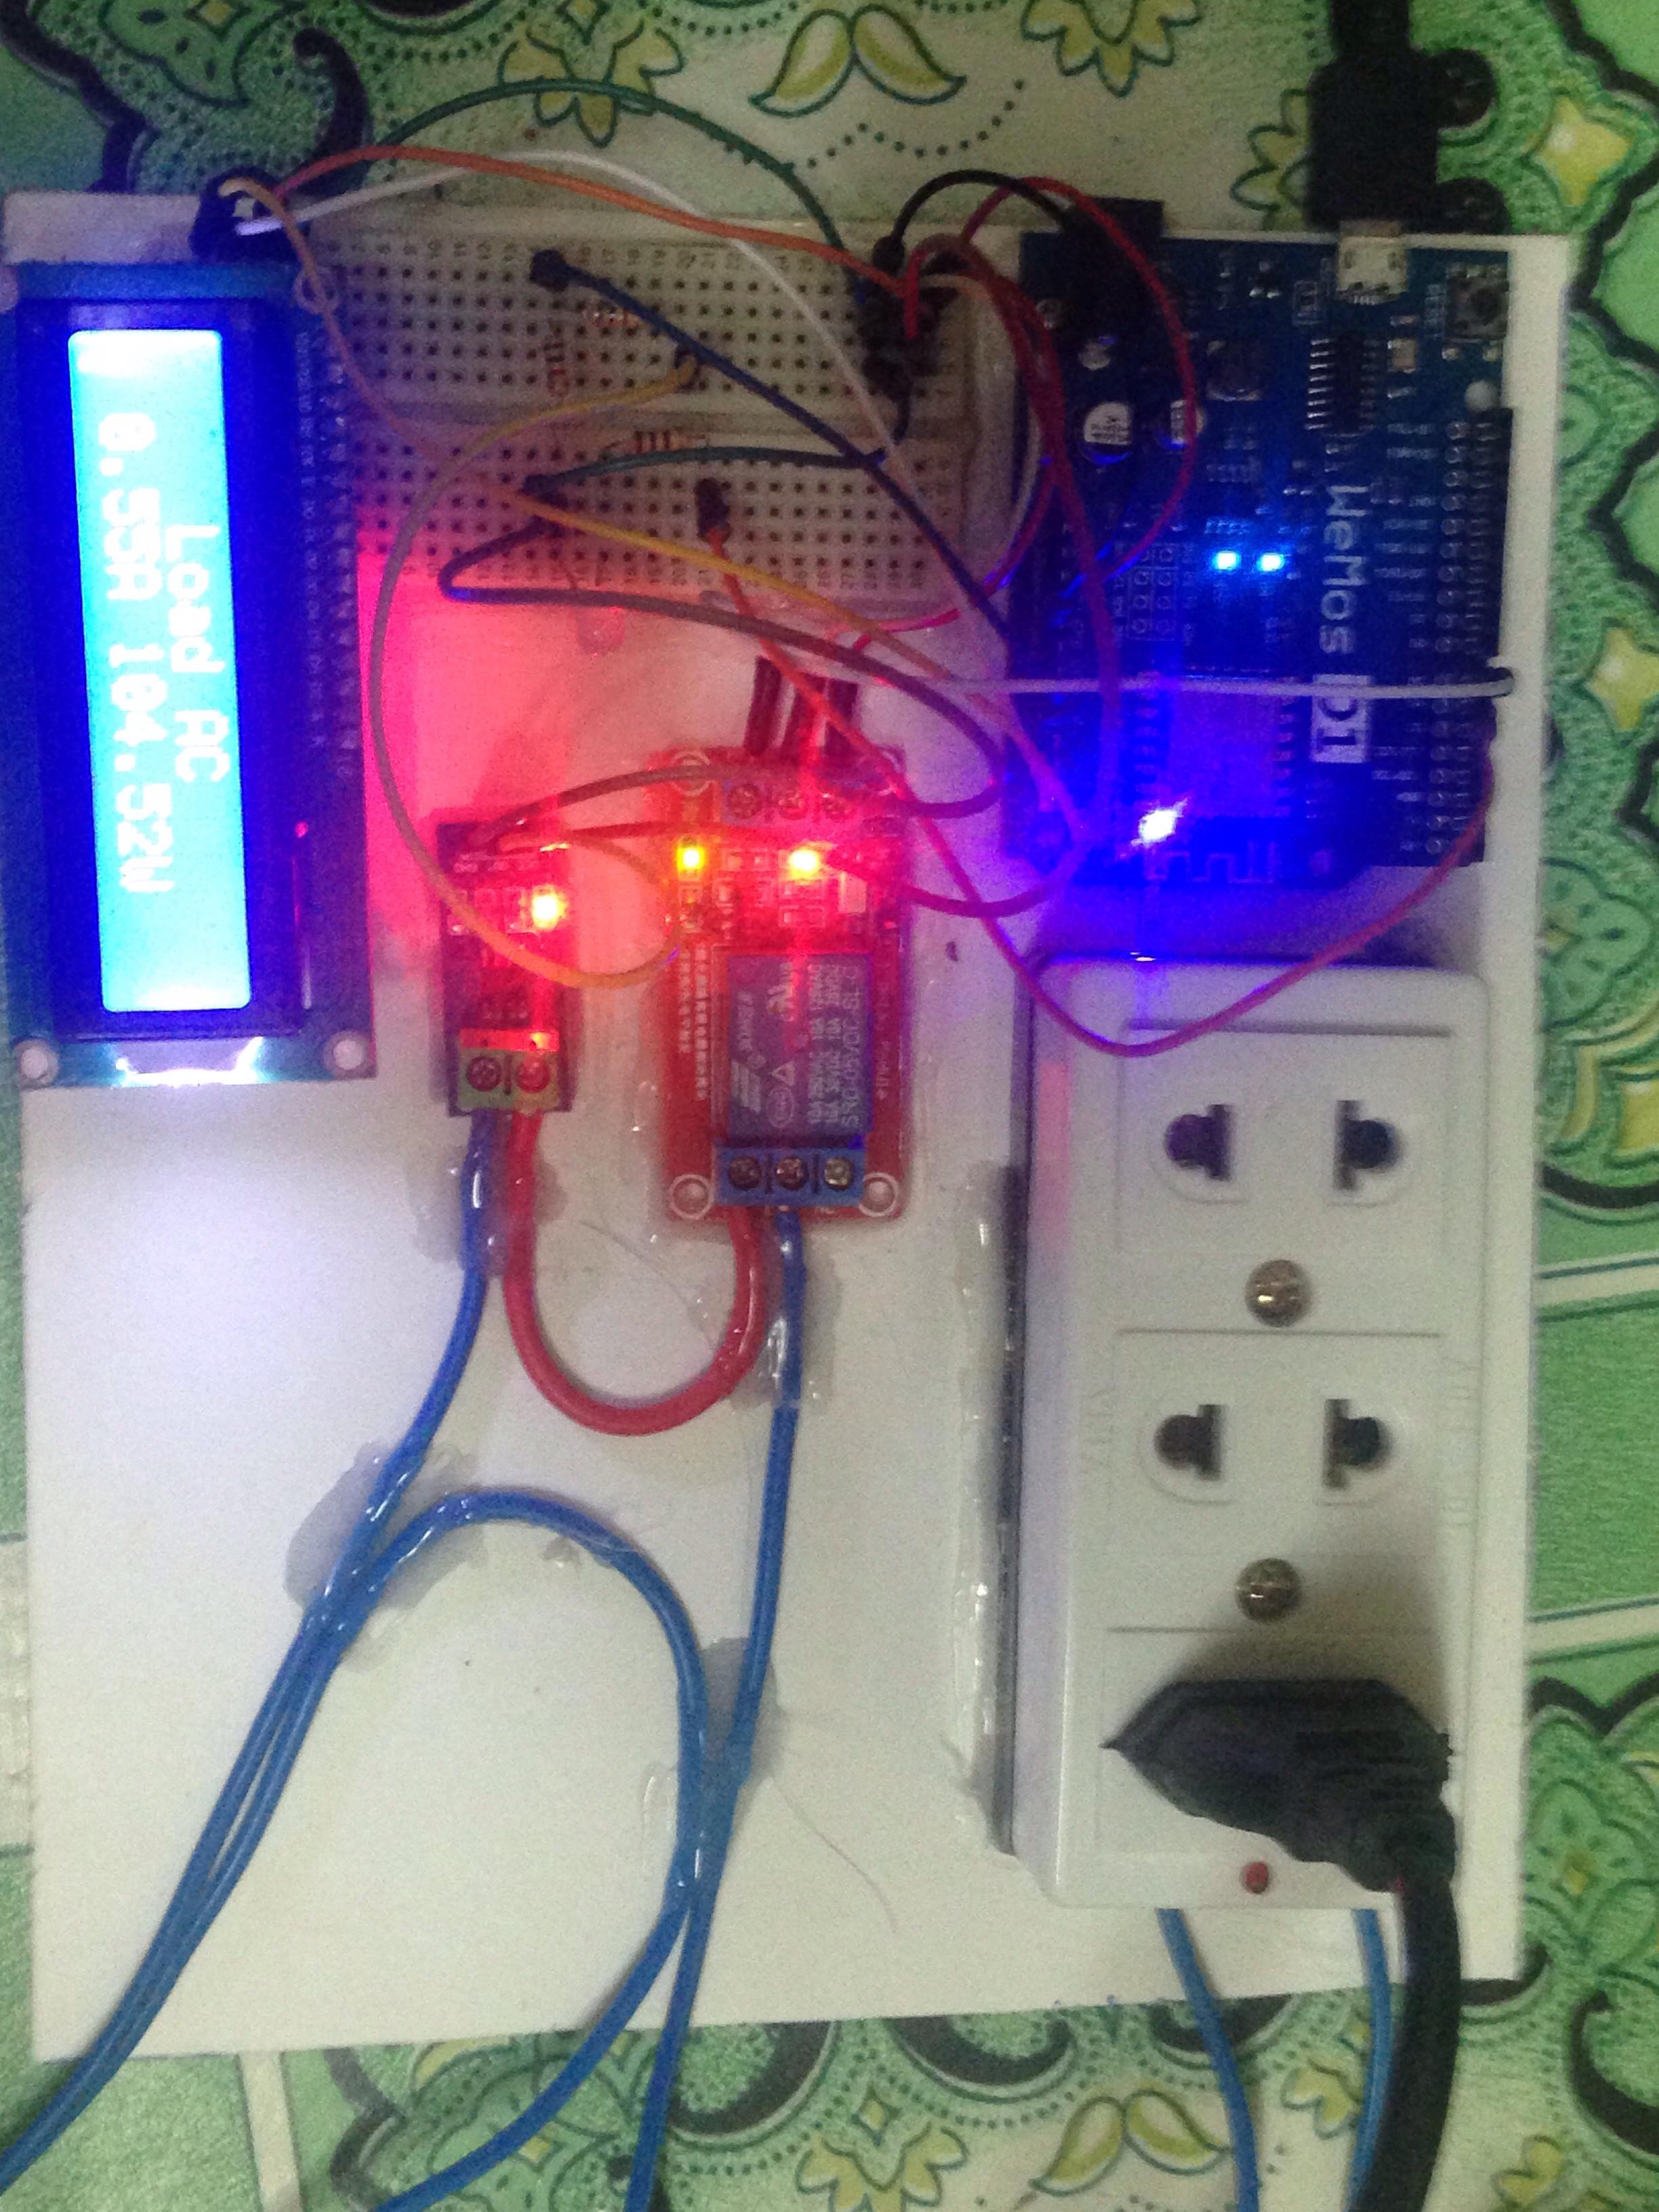
\includegraphics[scale=.08]{hardware-2}
        \end{center}
        \caption{Kết quả thu được về phần cứng} \label{Fig:result}
    \end{figure}

    \begin{figure}[htp]
        \begin{center}
            \subfloat[Kết quả trên Blynk]
                {
                    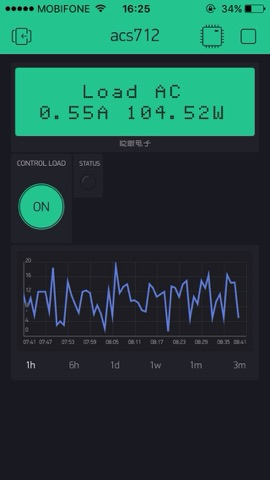
\includegraphics[scale=.5]{blynk-result}
                }
            \subfloat[Kết quả dòng điện trên Thingspeak]
                {
                    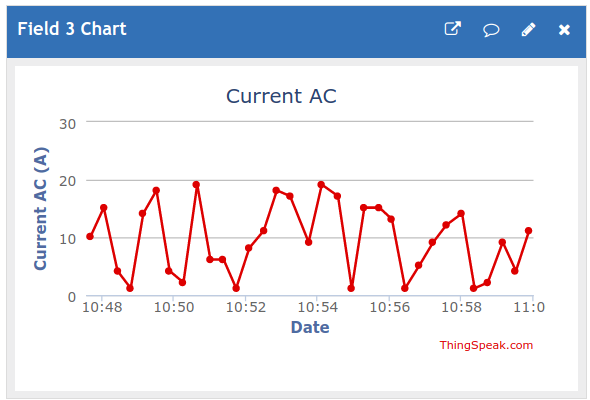
\includegraphics[scale=.5]{Current_Thingspeak}
                }\\

            \subfloat[Kết quả công suất trên Thingspeak]
                {
                    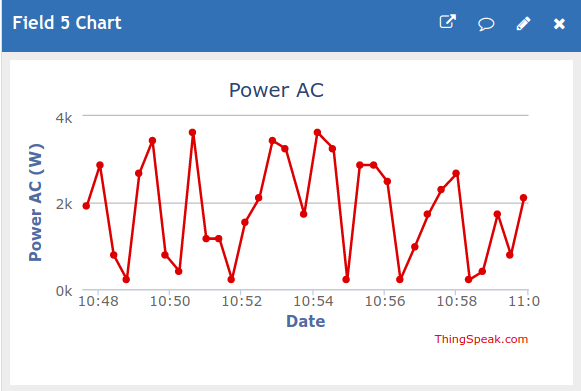
\includegraphics[scale=.35]{Power_Thingspeak}
                }
            \subfloat[Kết quả trạng thái quá tải trên Thingspeak]
                {
                    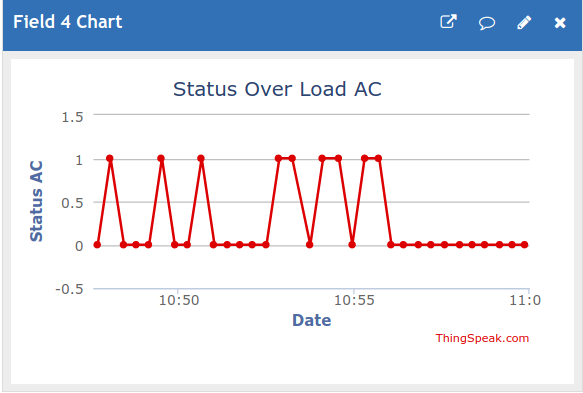
\includegraphics[scale=.35]{Status_Overload_Thingspeak}
                }
        \end{center}
        \caption{Kết quả thu được quan sát trên ứng dụng} \label{Fig:result}
    \end{figure}



    %----------------------------------------------------------------------------------------
    %    Chương 4 - Kết luận
    %----------------------------------------------------------------------------------------
    \chapter{KẾT LUẬN}

\section{Kết quả}
    Qua thời gian thực hiện đồ án, nhóm chúng em đạt được một số kết quả sau:
        \begin{itemize}
            \item Biết cách sử dụng module ESP8266 vào một số ứng dụng có kết nối WiFi.
            \item Điều khiển thiết bị từ xa và thu thập dữ liệu thông qua mạng WiFi với ứng dụng Blynk Web Server Thingspeak.
            \item Xây dựng ứng dụng theo dõi điện năng của phụ tải một pha với điều khiển và giám sát dữ liệu qua mạng Internet.
        \end{itemize}

\section{Hạn chế}
    Nhóm chúng em đã cố gắng tìm hiểu nhưng vẫn còn một số hạn chế sau:
        \begin{itemize}
            \item Chưa sử dụng nhiều tính năng của module ESP8266, App Blynk và Web Server Thingspeak.
            \item Trong ứng dụng theo dõi điện năng: chỉ đo một thông số là dòng điện tiêu thụ của phụ tải, cần kết hợp đo nhiều thông số hơn: điện áp, hệ số công suất, tần số dòng điện để có thể theo dõi chất lượng điện năng tốt hơn.
        \end{itemize}


    %----------------------------------------------------------------------------------------
    %    Tài liệu tham khảo
    %----------------------------------------------------------------------------------------
    %----------------------------------------------------------------------------------------
%
%    Tài liệu tham khảo
%
%----------------------------------------------------------------------------------------

    \begin{thebibliography}{9}
        \addcontentsline{toc}{chapter}{\textbf{TÀI LIỆU THAM KHẢO}}
            \bibitem{iot_maker_vietnam} Internet Of Things (IoT) cho người mới bắt đầu, IoT Maker Việt Nam.
            \bibitem{ac_current} AC current measurement using acs712 hall effect current sensor and Arduino, Microcontrollers Lab.
            \bibitem{dc_current} DC current measurement using acs712 hall effect current sensor and Arduino, Microcontrollers Lab.
            \bibitem{ThingSpeak} ThingSpeak, Blynk Examples.
    \end{thebibliography}


    % Tạo một trang trống cuối quyển đồ án
    % \NewPage
\end{document}
